Sebagaimana dijelaskan pada Subbab~3.9, \textit{minimum clearance} dipilih sebagai metrik uta\-ma dalam penelitian ini karena secara langsung merepresentasikan margin keselamatan yang dipertahankan robot terhadap obstacle selama proses navigasi berlangsung. Berbeda dengan \textit{success rate} yang hanya menunjukkan hasil akhir navigasi, \textit{minimum clearance} mampu mengg\-ambarkan tingkat risiko kolisi yang dialami robot sepanjang lintasan yang ditempuh.

Pada penelitian ini, nilai \textit{minimum clearance} dihitung sebagai jarak bebas minimum antara batas luar robot dan obstacle terdekat yang teramati selama satu percobaan. Semakin besar nilai \textit{minimum clearance}, semakin besar pula margin keselamatan yang dipertahankan robot ketika bergerak menuju tujuan.

\subsection{Perbandingan Minimum Clearance}

Nilai rata-rata \textit{minimum clearance} pada seluruh skenario ditunjukkan pada Tabel~\ref{tab:min_clearance}.

\begin{table}[H]
\centering
\caption{Perbandingan nilai minimum clearance pada seluruh skenario pengujian.}
\label{tab:min_clearance}
\begin{tabular}{ccc}
\toprule
Skenario & Konfigurasi & Minimum Clearance (m) \\
\midrule
S1 & Baseline & 0.0000 \\
S2 & Baseline & 0.4301 \\
S3 & Baseline & 0.0346 \\
S4 & Baseline & -0.1635 \\
S5 & Fuzzy & 0.0000 \\
S6 & Fuzzy & 0.4370 \\
S7 & Fuzzy & 0.1825 \\
S8 & Fuzzy & 0.3167 \\
\bottomrule
\end{tabular}
\end{table}

\begin{figure}[H]
\centering
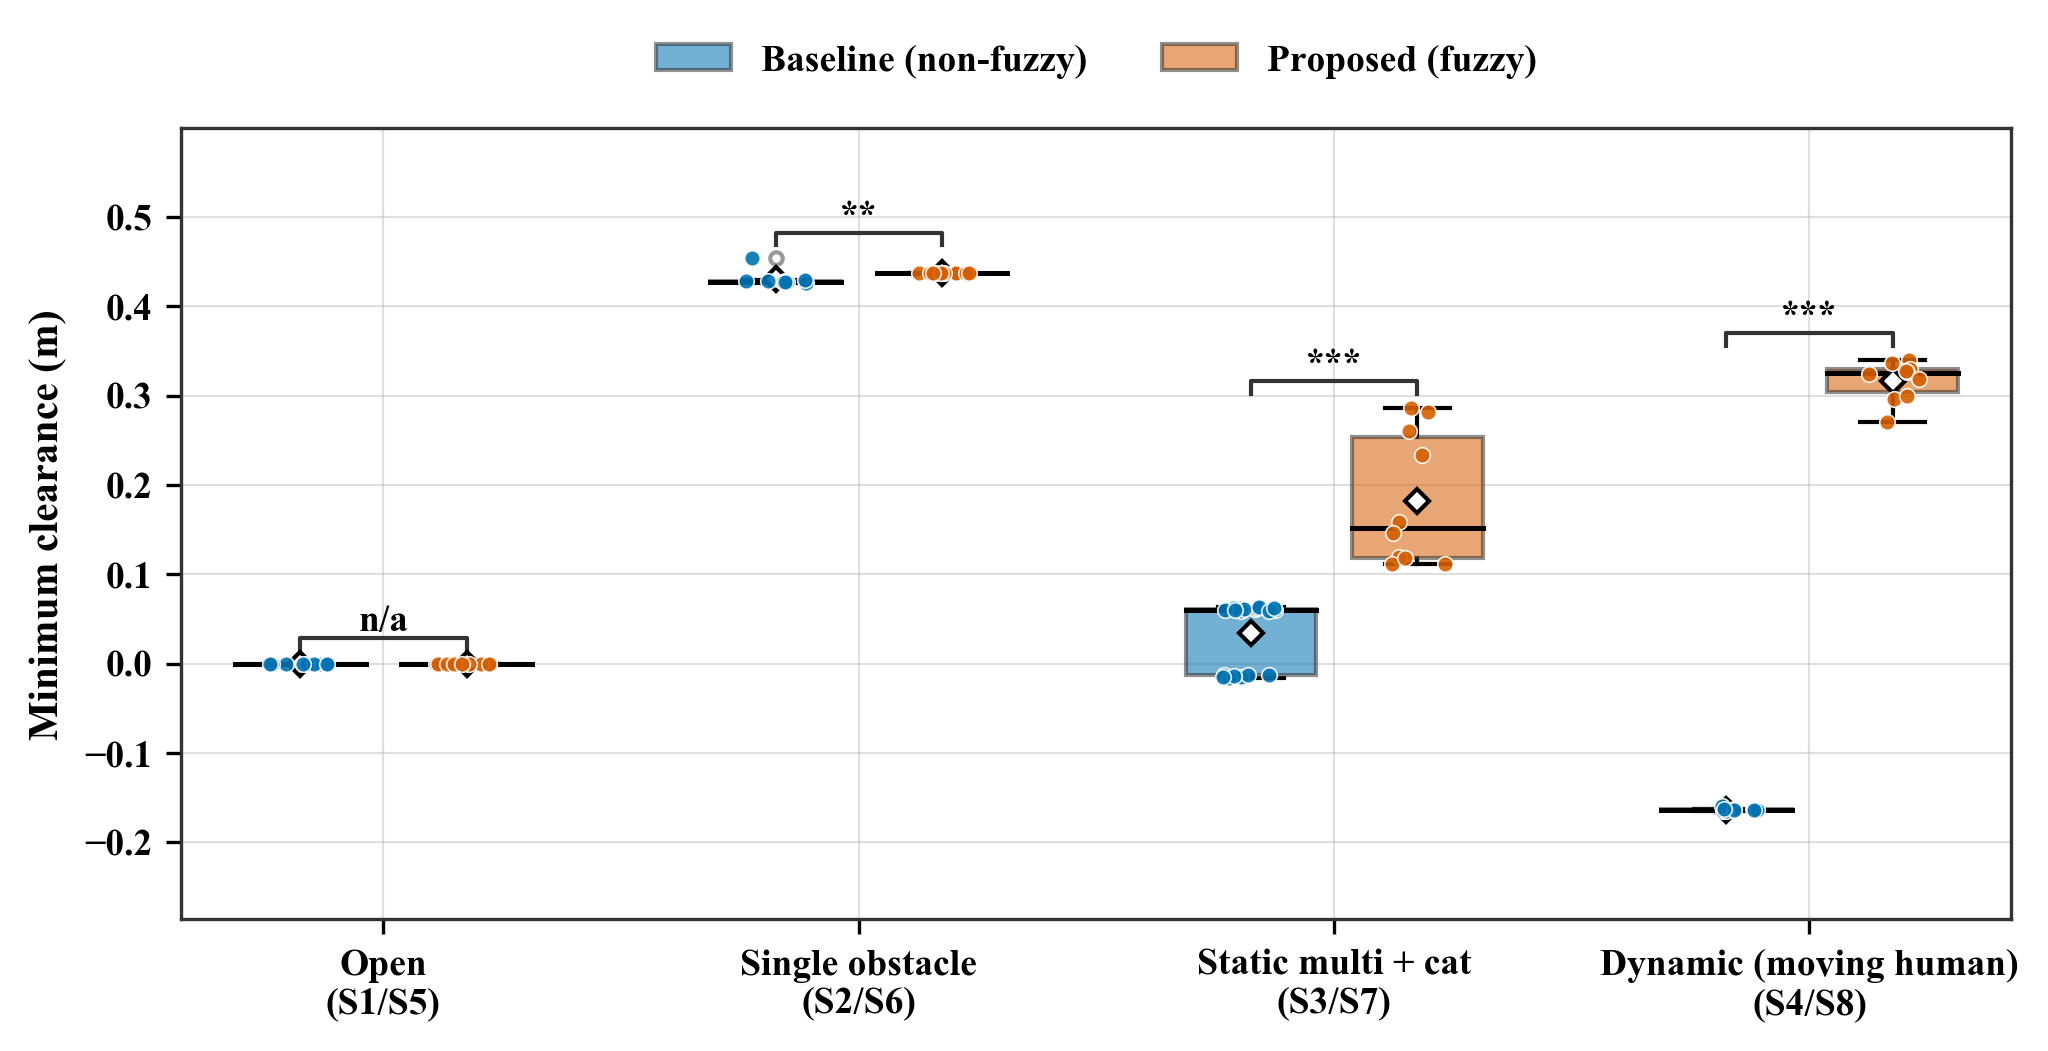
\includegraphics[width=0.7\textwidth]{gambar/4.4_fig_clearance_mean.png}
\caption{Perbandingan rata-rata minimum clearance pada seluruh skenario pengujian.}
\label{fig:mean_clearance}
\end{figure}

Secara umum, konfigurasi fuzzy menghasilkan nilai \textit{minimum clearance} yang lebih tinggi dibandingkan konfigurasi baseline pada seluruh pasangan skenario yang mengandung obstacle. Perbedaan tersebut relatif kecil pada lingkungan sederhana, namun meningkat secara signifikan ketika robot beroperasi pada lingkungan yang mengandung obstacle berprofil rendah dan obstacle dinamis.

Pada pasangan S2--S6, nilai \textit{minimum clearance} meningkat dari 0,4301~m menjadi 0,4370\\~m. Peningkatan ini relatif kecil karena kedua konfigurasi sama-sama mampu mendeteksi obstacle manusia yang berada dalam jangkauan observasi LiDAR. Oleh karena itu, kontribusi kamera termal dan mekanisme fuzzy belum terlihat secara dominan pada skenario ini.

Perbedaan yang lebih jelas terlihat pada pasangan S3--S7. Pada konfigurasi baseline, robot hanya mampu mempertahankan \textit{minimum clearance} sebesar 0,0346~m. Nilai tersebut menunjukkan bahwa robot bergerak sangat dekat dengan obstacle selama navigasi berlangsung. Setelah mekanisme fuzzy diaktifkan, nilai \textit{minimum clearance} meningkat menjadi 0,1825~m atau lebih dari lima kali lipat dibandingkan konfigurasi baseline.

Peningkatan yang paling signifikan terjadi pada pasangan S4--S8. Pada konfigurasi baseline, nilai \textit{minimum clearance} bernilai negatif sebesar -0,1635~m. Nilai negatif menunjukkan bahwa robot mengalami kontak dengan obstacle selama navigasi. Sebaliknya, konfigurasi fuzzy mampu mempertahankan \textit{minimum clearance} positif sebesar 0,3167~m sehingga seluruh percobaan dapat diselesaikan tanpa tabrakan. Hasil ini menunjukkan bahwa metode yang diusulkan mampu meningkatkan margin keselamatan secara substansial pada lingkungan dengan tingkat kompleksitas tinggi.

\subsection{Distribusi Minimum Clearance}

Untuk memperoleh gambaran yang lebih komprehensif mengenai penyebaran data, distribusi \textit{minimum clearance} pada setiap pasangan skenario divisualisasikan menggunakan boxplot sebagaimana ditunjukkan pada Gambar~\ref{fig:boxplot_clearance}.

\begin{figure}[H]
\centering
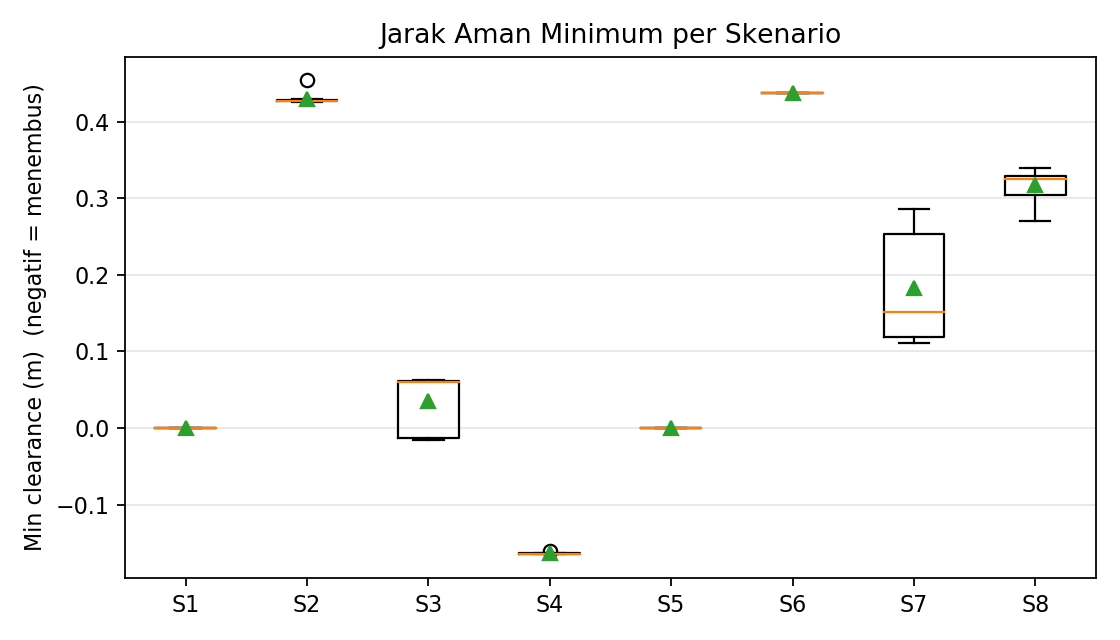
\includegraphics[width=0.9\textwidth]{gambar/4.4_fig_clearance_box.png}
\caption{Distribusi minimum clearance pada seluruh pasangan skenario pengujian.}
\label{fig:boxplot_clearance}
\end{figure}

Distribusi data pada Gambar~\ref{fig:boxplot_clearance} menunjukkan bahwa konfigurasi fuzzy tidak hanya meni\-ngkatkan nilai rata-rata \textit{minimum clearance}, tetapi juga menggeser keseluruhan distribusi data menuju nilai clearance yang lebih tinggi. Pergeseran tersebut terlihat paling jelas pada pasangan S3--S7 dan S4--S8 yang merepresentasikan lingkungan dengan tingkat kompleksitas tinggi.

Pada pasangan S3--S7, sebagian besar percobaan pada konfigurasi baseline menghasilkan clearance yang sangat kecil sehingga robot bergerak dalam jarak yang sangat dekat terhadap obstacle. Setelah mekanisme fuzzy diaktifkan, distribusi data bergeser ke arah nilai yang lebih besar dan menunjukkan bahwa robot secara konsisten mempertahankan jarak aman selama navigasi berlangsung.

Fenomena yang lebih menonjol terlihat pada pasangan S4--S8. Distribusi data pada S4 menunjukkan adanya sejumlah percobaan dengan nilai clearance negatif yang mengindikasikan terjadinya tabrakan. Sebaliknya, seluruh distribusi pada S8 berada pada daerah clearance positif dengan median yang jauh lebih tinggi. Hasil tersebut menunjukkan bahwa metode yang diusulkan tidak hanya meningkatkan rata-rata clearance, tetapi juga menghilangkan kejadian tabrakan yang sebelumnya muncul pada konfigurasi baseline.

\subsection{Analisis Statistik Minimum Clearance}

Untuk mengevaluasi apakah perbedaan yang diamati bersifat signifikan secara statistik, dilakukan uji Mann--Whitney U terhadap setiap pasangan skenario yang memiliki kondisi lingku\-ngan identik. Hasil pengujian ditunjukkan pada Tabel~\ref{tab:mw_clearance}.

\begin{table}[H]
\centering
\caption{Hasil uji Mann--Whitney U untuk minimum clearance.}
\label{tab:mw_clearance}
\begin{tabular}{cccc}
\toprule
Pasangan &
$p$-value &
Effect Size ($r$) &
Interpretasi \\
\midrule
S1--S5 & n/a & n/a & Tidak berbeda \\
S2--S6 & 0.0013 & 0.80 & Besar \\
S3--S7 & $<0.001$ & 1.00 & Sangat besar \\
S4--S8 & 0.0002 & 1.00 & Sangat besar \\
\bottomrule
\end{tabular}
\end{table}
Hasil uji Mann--Whitney U menunjukkan bahwa peningkatan
\textit{minimum clearance} pada konfigurasi fuzzy bersifat
signifikan secara statistik pada seluruh skenario yang
mengandung obstacle. Pada pasangan S2--S6 diperoleh
$p=0.0013$ dengan \textit{effect size} sebesar $r=0.80$,
yang termasuk kategori besar. Meskipun peningkatan
clearance pada skenario ini relatif kecil secara absolut,
hasil tersebut menunjukkan bahwa konfigurasi fuzzy secara
konsisten mempertahankan jarak aman yang lebih tinggi
dibandingkan konfigurasi baseline.

Perbedaan yang lebih kuat terlihat pada pasangan S3--S7
dan S4--S8. Pada kedua pasangan tersebut diperoleh
nilai $p<0.001$ dengan \textit{effect size} sebesar
$r=1.00$, yang menunjukkan perbedaan sangat besar antara
kedua kelompok. Hasil ini mengindikasikan bahwa seluruh
distribusi data pada konfigurasi fuzzy bergeser menuju
nilai clearance yang lebih tinggi dibandingkan konfigurasi
baseline.

Temuan tersebut memperkuat hasil deskriptif yang telah
ditunjukkan pada subbab sebelumnya. Pada lingkungan yang
mengandung obstacle berprofil rendah dan obstacle dinamis,
integrasi kamera termal memungkinkan sistem mendeteksi
hambatan yang tidak sepenuhnya teramati oleh LiDAR 2D,
sementara pengendali fuzzy menyesuaikan parameter
\textit{speed scale} dan \textit{repulsive gain}
secara adaptif ketika tingkat traversability menurun.
Kombinasi kedua mekanisme tersebut menghasilkan peningkatan
margin keselamatan yang signifikan dan konsisten pada
berbagai kondisi pengujian.

Berdasarkan hasil tersebut, hipotesis H1 yang menyatakan
bahwa metode usulan menghasilkan nilai \textit{minimum clearance}
yang lebih tinggi dibandingkan konfigurasi baseline dapat
diterima.